\chapter{Introducción Específica} % Main chapter title

\label{Chapter2}

Es este capítulo se presentarán las topologías básicas del sistema ferroviario y los dos enfoques de resolución del proyecto, con sus ventajas y desventajas antes de abordar la implementación de la solución elegida.

\section{Topologías típicas}
	
	El tendido ferroviario argentino dista de ser uniforme: en las zonas rurales predominan vías simples con bypass debido al alto costo de utilizar vías dobles, mientras que en las zonas urbanas son mayoría las estaciones y playas de maniobras a talleres de mantenimiento.
	
	Es por eso que el trabajo realizado debe abocarse a muchos frentes y muy diversos unos de otros. La cantidad de elementos involucrados diverge conforme la complejidad de la topología se incrementa, pero los elementos y sus comportamientos no dejan de ser los mismos de los presentados en el Capítulo 1.

	\subsection{Bypass}

		Para cubrir grandes distancias entre un punto estratégico como podría ser Vaca Muerta y un puerto para la exportación de los recursos es necesaria una línea ferroviaria con vagones de carga que puedan transportar el producto. Es obvio que es necesario un ida y vuelta entre trenes vacíos que van a ser llenados en el destino y trenes llenos que van a descargar al puerto la carga que lleven, pero el costo de utilizar dos vías en sentidos opuestos es muy elevado y utilizar solo un no tiene el menor sentido logístico.
		
		Es por eso que se utiliza la topología de bypass cada cierta cantidad de kilómetros de vía simples para poder permitir que trenes en sentidos opuestos se crucen sin riesgo de colisión. Se presenta en la figura \ref{fig:Bypass} una representación de la topología bypass donde un tren que circula hacia la derecha por la vía principal podría entrar en colisión lateral con un tren que busca ingresar a la red desde una vía secundaria por medio del cambio de vías.
		
		\begin{figure}[h]
		\centering
			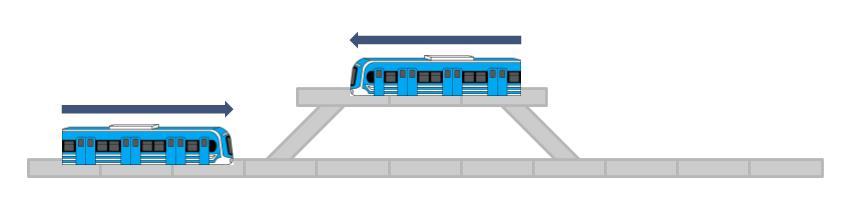
\includegraphics[scale=.5]{./Figures/Bypass_2}
			\caption{Topología bypass.}
			\label{fig:Bypass}
		\end{figure}

	\vspace{5cm}
				
	\subsection{Estación}

		Los lugares donde se habilita a los pasajeros a ingresar o salir del tren se denominan andenes y se encuentran en las estaciones ferroviarias situadas cada cierta cantidad de kilómetros, en diferentes localidades del país. En la figura \ref{fig:Estacion} se muestra una topología de estación simple con andén central. Es decir, el mismo andén permite utilizar trenes tanto de la vía ascendente como de la descendente. Se añadió un paso a nivel vehicular en las inmediaciones de la estación y dos cambios de vías en orientaciones opuestas para permitir a la hipotética estación realizar trayectos cortos entre terminales.
		
			\begin{figure}[h]
			\centering
				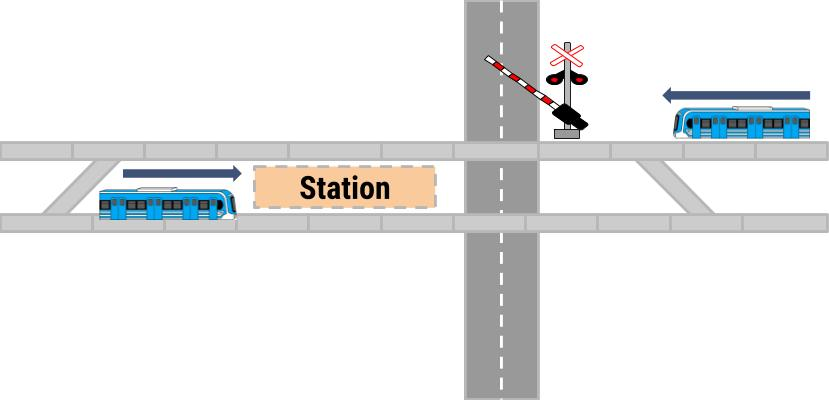
\includegraphics[scale=.5]{./Figures/Estacion}
				\caption{Topología estación con andén único.}
				\label{fig:Estacion}
			\end{figure}
		
		Aunque estaciones de andén único como la estación de Gerli de la Línea Roca son comunes, también existen estaciones con dos andenes: uno puramente para utilizar la vía ascendente y alejarse de la terminal y otro puramente descendente para viajar hacia la terminal. Tal es el caso de estaciones como Longchamps, Adrogué, Remedios de escalada de la Línea Roca.

	\subsection{Hub}
	
		Otras topologías mas complejas incluyen una cantidad extra de andenes como Lomas de Zamora o Temperley, que pueden recibir formaciones de varios ramales distintos (Glew/A.Korn, Ezeiza, Bosques, Quilmes, La Plata, etc) o tener incluso accesos a playas de maniobras o talleres de reparación para poder inyectar o retirar formaciones de la red. Tal es el caso representado en la figura \ref{fig:Hub} donde se tiene una mayor cantidad de andenes, bifurcaciones a otros ramales o ingresos/egresos a talleres ferroviarios, además de la rama principal de circulación entre terminales. 
		
			\begin{figure}[h]
			\centering
				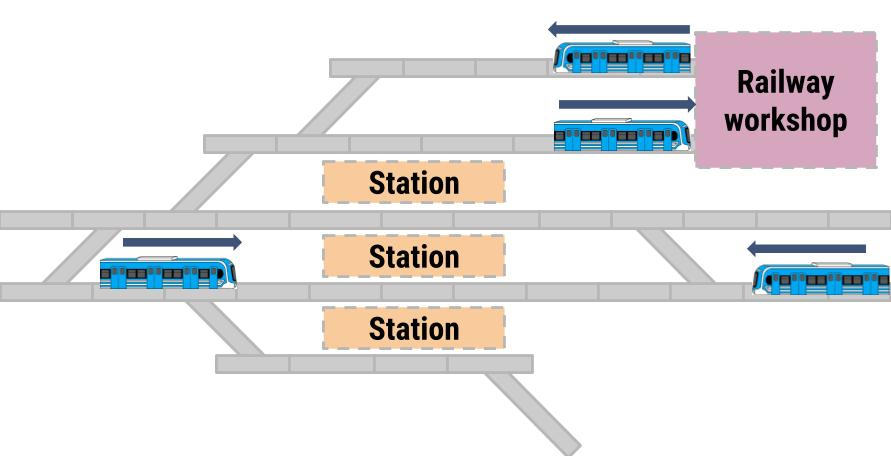
\includegraphics[scale=.45]{./Figures/Hub}
				\caption{Topología hub.}
				\label{fig:Hub}
			\end{figure}
	
		Un buen ejemplo de esta topología es la estación Llavallol de la Línea Roca. En la misma se tiene una extensa playa de maniobras como la comandada por el panel de control de la figura \ref{fig:Electromecanico} mostrada en la Sección 1.
		
	\subsection{Terminal}
		
		Finalmente, la topología mas compleja de todas es la denominada terminal, tal como se representa en la figura \ref{fig:Terminal}. En las mismas se encuentran numerosos andenes que pueden ser tanto de ingreso como de egreso indistintamente, presentan muchos cambios de vías para facilitar el intercambio de formaciones y permitir que las vías funcionen en ambos sentidos de circulación. Además de tener ramificaciones para diversos ramales que convergen en la terminal.
		
			\begin{figure}[h]
			\centering
				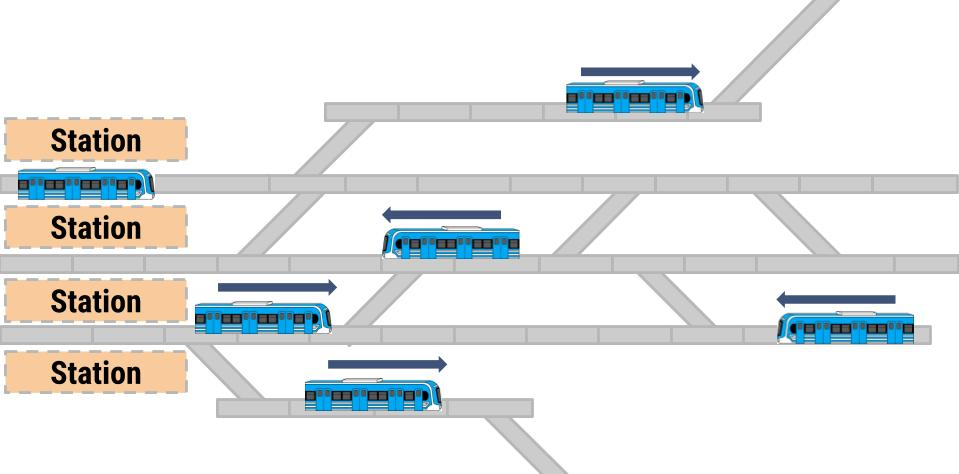
\includegraphics[scale=.4]{./Figures/Terminal}
				\caption{Topología terminal.}
				\label{fig:Terminal}
			\end{figure}
		
		Ejemplos de esta topología pueden ser las estaciones Once de septiembre(Línea Sarmiento), Alejandro Korn y Constitución (Línea Roca) o Retiro (Línea San Martín, Línea Mitre, Línea Belgrano Norte y Cargas). Incluso hay estaciones que aunque no son el final del recorrido, pueden funcionar como terminales de ramales mas cortos tales como Ezeiza, que extiende el ramal Constitución-Ezeiza hasta Cañuelas o Glew, que extiende el ramal Constitución Glew hasta Alejandro Korn.
							
\section{Enfoque funcional}
	\label{Incompletitud}
	
	A la hora de definir itinerarios se utiliza el concepto de ruta, que es el camino definido entre dos semáforos consecutivos. Pero no siempre se suelen definir todas las rutas posibles, sino solo las necesarias para generar los itinerarios. Por ejemplo en la figura \ref{fig:EJ_Tabla} se pueden ver dos casos de definición de rutas para una misma topología de vía simple.
	
	\begin{figure}[h]
		\centering
			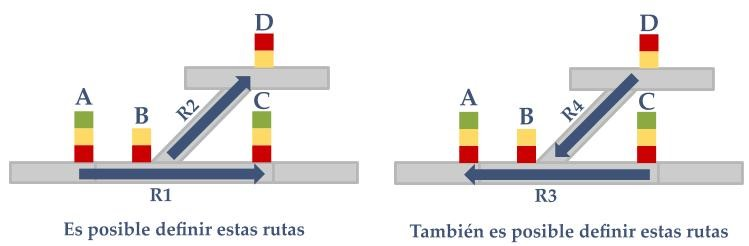
\includegraphics[scale=.4]{./Figures/Tablas}
			\caption{Ejemplo de elaboración de tabla de enclavamientos.}
			\label{fig:EJ_Tabla}
		\end{figure}
	
	En el primer caso se puede querer utilizar la vía en un solo sentido, para lo cual el semáforo A es el inicial de la ruta $\text{R}_1$ y el semáforo B es el final de la misma. Luego se definen las otras dos rutas y el itinerario para recorrer toda la topología es la concatenación de las rutas $\text{R}_1$,$\text{R}_2$ y $\text{R}_3$ como se describen en la Tabla \ref{Tabla_simple}.
	
	\begin{table}[!hbt]
	\renewcommand{\arraystretch}{1.3}

	\caption{Tabla de enclavamientos(caso unidireccional)}
	\label{Tabla_simple}
	\centering

	\begin{tabular}{c c c c c c c}
	\hline
	Ruta & Señal de entrada & Señal de salida \\
	\hline
	 1 & $\text{Semáforo}_A$  & $\text{Semáforo}_B$ \\
	 2 & $\text{Semáforo}_B$  & $\text{Semáforo}_C$ \\
	 3 & $\text{Semáforo}_C$  & $\text{Semáforo}_D$ \\
	\hline
	\end{tabular}
	\end{table}
	
	En el segundo caso de la figura \ref{fig:EJ_Tabla} el itinerario deberá contemplar un uso bidireccional de la vía, por lo que se añaden las rutas $\text{R}_4$,$\text{R}_5$ y $\text{R}_6$ como se describen en la Tabla \ref{Tabla_bidireccional}
	
	\begin{table}[!hbt]
	\renewcommand{\arraystretch}{1.3}

	\caption{Tabla de enclavamientos(caso bidireccional)}
	\label{Tabla_bidireccional}
	\centering

	\begin{tabular}{c c c c c c c}
	\hline
	Ruta & Señal de entrada & Señal de salida \\
	\hline
	 1 & $\text{Semáforo}_A$  & $\text{Semáforo}_B$ \\
	 2 & $\text{Semáforo}_B$  & $\text{Semáforo}_C$ \\
	 3 & $\text{Semáforo}_C$  & $\text{Semáforo}_D$ \\
	 4 & $\text{Semáforo}_B$  & $\text{Semáforo}_A$ \\
	 5 & $\text{Semáforo}_C$  & $\text{Semáforo}_B$ \\
	 6 & $\text{Semáforo}_D$  & $\text{Semáforo}_C$ \\
	\hline
	\end{tabular}
	\end{table}
	
	\vspace{5cm}
	
	Tanto la Tabla \ref{Tabla_simple} como la \ref{Tabla_bidireccional} son una porción de la llamada tabla de enclavamientos, que se utiliza para diseñar los sistemas de enclavamientos tanto mecánicos como electromecánicos y define completamente el comportamiento del sistema. En la misma cada ruta constituye una fila y presenta diferentes columnas tales como:
	
	\begin{itemize}
		\item Semáforos de entrada y de salida.
		\item Circuitos de vías que deben estar desocupados para permitir la ruta.
		\item Pasos a nivel que deben tener la barrera baja para permitir la ruta.
		\item Posición del cambio requerida para permitir la ruta.
		\item Rutas conflictivas que inhiben la activación de la ruta.
	\end{itemize}
	
	Como se pudo ver en ambos ejemplos, la necesidad de tales o cuales itinerarios puede requerir distintas tablas de enclavamientos para la misma topologías. Algunas tablas serán mas completas que otras y eso puede repercutir en que al querer añadir nuevas rutas a futuro, la tabla deba ser modificada y por lo tanto el desarrollo del sistema deba cambiar a otro mas complejo.
	
	\subsection{Modelo del sistema}
		
		En el enfoque de desarrollo llamado funcional se utiliza la tabla de enclavamientos como elemento central de decisión para el diseño y funcionamiento del sistema. Es la ruta la que impone que acciones deben ser tomadas y cuales prohibidas y por lo tanto se abstrae de la topología una vez definida la tabla.
			
		En la figura \ref{fig:Modelo_Funcional} se presenta un modelo del sistema con enfoque funcional, donde cada bloque horizontal en diferentes colores representan máquinas de estados que modelan los elementos de entrada indicados. Todos ellos gobernados por una máquina de estados general representada en un bloque vertical verde que se diseña en base a la tabla de enclavamientos. 	
		
			\begin{figure}[h!]
			\centering
				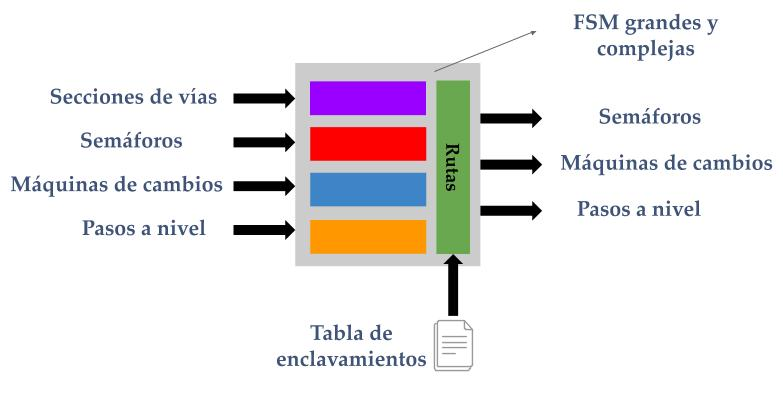
\includegraphics[scale=.55]{./Figures/Funcional}
				\caption{Enfoque funcional.}
				\label{fig:Modelo_Funcional}
			\end{figure}
		
		\vspace{5cm}
			
		La salida del sistema actúa sobre todo el señalamiento, menos la ocupación de los tramos de vías porque son elementos de solo lectura. Puede verse que conforme se añadan mas rutas a la tabla de enclavamientos, las máquinas de estados serán mas complejas y de mayor tamaño.
	
	\subsection{Flujo de trabajo}
		
		La tabla de enclavamientos es la piedra angular de todo el proceso, sin ella no se puede realizar ningún diseño. En la figura \ref{fig:Work_Funcional} se ilustra el flujo de trabajo en el enfoque funcional.		
			
		\begin{figure}[h]
		\centering
			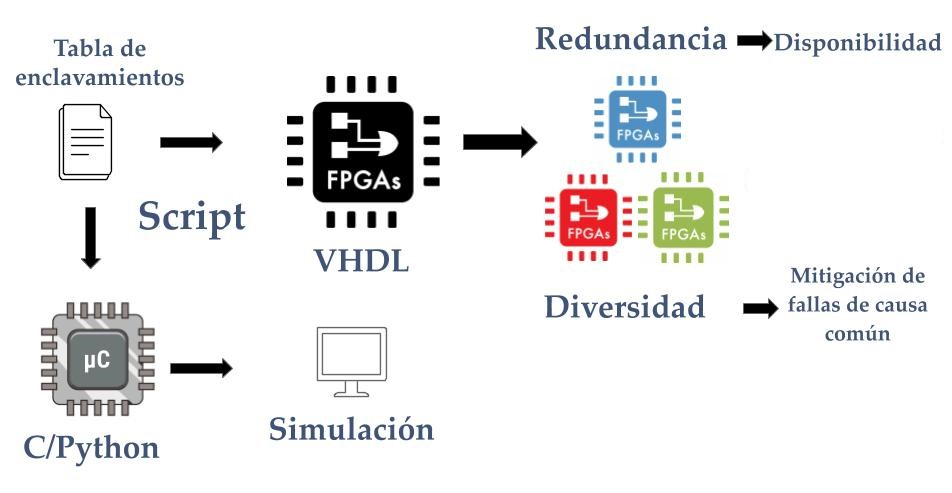
\includegraphics[scale=.4]{./Figures/Funcional_workflow}
			\caption{Esquema de trabajo en el enfoque funcional.}
			\label{fig:Work_Funcional}
		\end{figure}
	
		Como bien se resaltó anteriormente, el diseño nace de la tabla de enclavamientos y para evitar que cualquier error en la misma se propague al sistema, la tabla es diseñada y revisada por varios profesionales ferroviarios. Pero si aún así no es suficiente, en la UTN-Haedo se ha avanzado en el desarrollo de un script que busca errores en las tablas de enclavamientos.
		
		El proceso culmina con la redundancia de los sistemas diseñados y la diversificación de plataformas, sin lo cual no se podría alcanzar estándares de calidad y seguridad altos como los demandados por industrias tan críticas como la nuclear, la aeronáutica, etc. 
		
		En el transcurso de la Especialización de Sistemas Embebidos se trabajó en un diseño con enfoque funcional de la estación Belgrano R de la Línea Mitre, pero sin automatización del proceso. En el cual la tabla de enclavamientos fue una pieza vital de todo el desarrollo.
		
		Durante 2019 se avanzó en la automatización de este flujo de trabajo, que culminó con la presentación de un artículo en el Congreso Argentino de Sistemas Embebidos 2019 y en una edición especial de IEEE Latin American Transaction.
		
	\subsection{Escalabilidad de la estrategia}	
		
		Al ir automatizando el sistema se fue llegando a la conclusión de que los bloques que contenían las máquinas de estados se crecían en tamaño hasta volverse inmanejables las conexiones. En la figura \ref{fig:Escala_Funcional} se representa el concepto del crecimiento del sistema conforme la topología se vuelve mas compleja.		
					
		\begin{figure}[h]
		\centering
			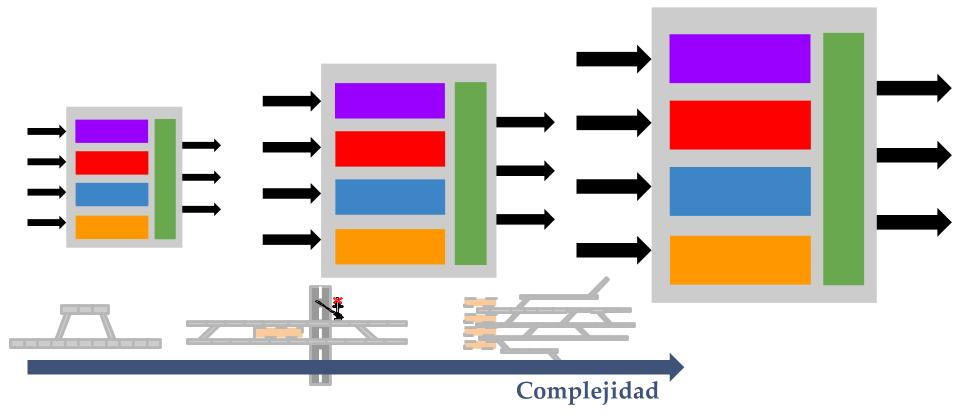
\includegraphics[scale=.4]{./Figures/Funcional_complejidad}
			\caption{Escalabilidad del enfoque funcional.}
			\label{fig:Escala_Funcional}
		\end{figure}
		
	Es destacable que a medida que la topología se complejiza la cantidad de bloques para modelarla sigue siendo la misma. Lo que incrementa es la cantidad de estados en cada máquina de estados y la densidad de conexiones tanto entre los bloques como internamente.
	
	El tener bloques monolíticos y de crecimiento exponencial perjudica el desarrollo de los tests que deben ser desechados y reescritos de cero cada vez que la topología cambie, por mas mínimos que sean los cambios. 
	
	Otro problema encontrado es el de la incompletitud, que se detallo al inicio de la Sección \ref{Incompletitud}. Si la red admite M rutas pero solo se definieron N como necesarias (donde $N \leq M$) entonces se podrían tener N tests que las validen y el sistema se certifica para N rutas. Pero si en un futuro se necesitan N+1 rutas se deberá hacer todo el proceso de validación desde cero, encareciendo todo el proyecto.
			
	La ventaja central de este enfoque es que, teniendo la tabla de enclavamientos correctamente definida, es muy sencillo e inmediato pasar de la tabla a la implementación del sistema. Aunque el uso de memoria es excesivo y desde el punto de vista del testing y la validación es incompleto.			
					
\section{Enfoque geográfico}

	En el mundo de la electrónica el concepto de red circuital se usa ampliamente. El funcionamiento de la red a nivel macro es la consecuencia directa de los principios físicos de funcionamiento de pequeños elementos discretos (resistores, capacitores, inductores, etc) y su interconexión entre ellos. Sabiendo como funciona un componente es posible predecir y simular el comportamiento de una red entera llena de estos, sin importar que sean de diferente valor, solo basta con que sean regidos por el mismo principio físico.
	
	Es entonces que removemos el concepto de ruta como elemento central del desarrollo y nos enfocamos a modelar los elementos discretos de la red ferroviaria (semáforos, barreras, cambios, circuitos de vía). Este enfoque se denomina geográfico, ya que el comportamiento macro de la red es consecuencia directa de la relación entre los elementos mencionados. En la figura \ref{fig:Enfoque_Geografico} se representa la idea central de este enfoque: la variedad de elementos es finita y puede ser modelada facilmente, el foco del desarrollo debe estar centrado en el análisis de la red ferroviaria misma.
	
		\begin{figure}[h]
		\centering
			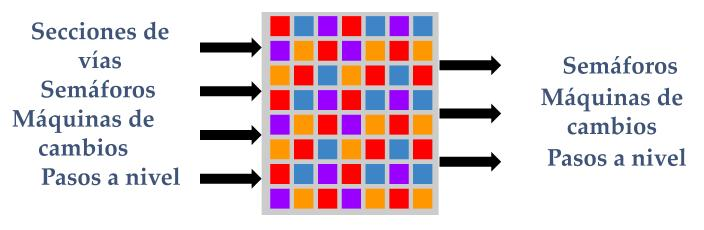
\includegraphics[scale=.55]{./Figures/Geografico}
			\caption{Enfoque geográfico.}
			\label{fig:Enfoque_Geografico}
		\end{figure}

	Se puede apreciar en la figura que la variedad de colores de los pequeños bloques es limitada. Esto se debe a que cada uno simboliza un elemento ferroviario, sin importar cual sea. El concepto a destacar es que una vez que se ha modelado un bloque rojo, todos los bloques rojos se comportarán igual y es su posición relativa a los otros bloques (sean o no rojos) lo que tendrá una funcionalidad a nivel general.
	
	\subsection{Análisis de grafos}
		
		Un grafo es una representación matemática de las relaciones (aristas) entre componentes (nodos) de una red. Utilizado ampliamente en ciencias de la computación y matemática, es sencillo llegar a un modelo de grafos partiendo desde una topología como la de la figura \ref{fig:Topologia_Grafo}, donde a cada tramo de vía se le asignó un nodo y cada arista del grafo representa el vínculo que existe entre ese tramo y sus vecinos.
		
		\begin{figure}[h]
		\centering
			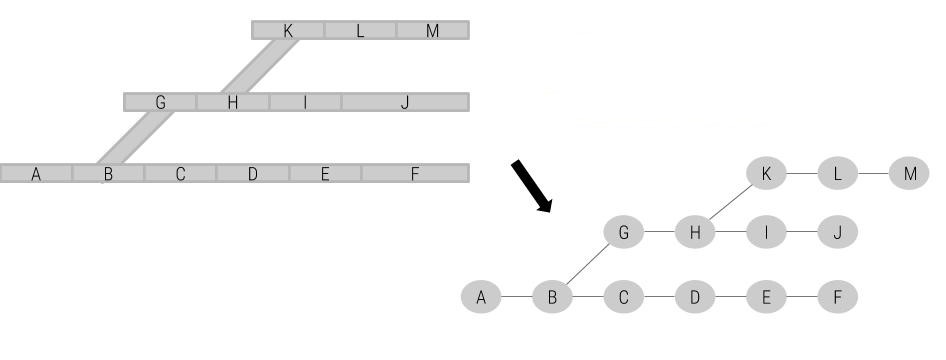
\includegraphics[scale=.4]{./Figures/Topologia_grafo}
			\caption{Pasaje de topología ferroviaria a grafo.}
			\label{fig:Topologia_Grafo}
		\end{figure}
	
		Por ejemplo, el nodo B posee un cambio de vías que vincula los tramos A y C si el cambio se encuentra en posición normal y los tramos A y G si el cambio se encuentra en posición inversa. Por lo tanto en el grafo, el nodo B posee aristas que lo vinculan con los nodos A,C y G.
		
		La misma topología de la figura \ref{fig:Topologia_Grafo} puede ser analizada por el algoritmo creado para este trabajo utilizando como información únicamente el grafo que la modela. Todos los nodos que tengan un solo vecino son extremos de la red, mientras que los que tengan tres vecinos se asumirá que poseen un cambio de vías. Los nodos que tengan dos vecinos serán analizado según su posición relativa a cambios cercanos. El resultado de analizar esta topología se muestra en la figura \ref{fig:Grafo_Analisis}.
	
		\begin{figure}[h]
		\centering
			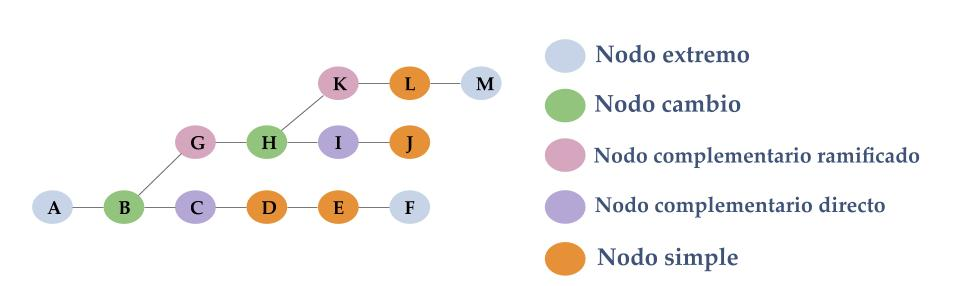
\includegraphics[scale=.4]{./Figures/Grafo}
			\caption{Análisis del grafo ferroviario.}
			\label{fig:Grafo_Analisis}
		\end{figure}
	
		Nodos como el G y el K deben analizarse por su posición relativa a los nodos B y H que son la raíz del cambio. Al desprenderse de la rama principal de circulación son categorizados como complementos de rama. En cambio los nodos C e I al continuar el trayecto que tienen los nodos A-B y G-H son complementos directos de la rama, porque la extienden mas allá de los segmentos indicados.
		
		Otros nodos como D,E y L no tienen ninguna caracteristica especial en este ejemplo, pero bien podrían categorizarse de otra manera si por los tramos de vías que representan se tuviese un paso a nivel.
	
		\subsection{Flujo de trabajo}
		
		El procedimiento se puede repetir infinitamente para cualquier topología, ya que sin importar la cantidad de elementos o sus conexiones, todos los vínculos entre componentes pueden ser representados mediante un grafo. Se ilustra en la figura \ref{fig:Work_Geografico} el esquema de trabajo seguido para el enfoque geográfico.	
		
		\begin{figure}[h]
		\centering
			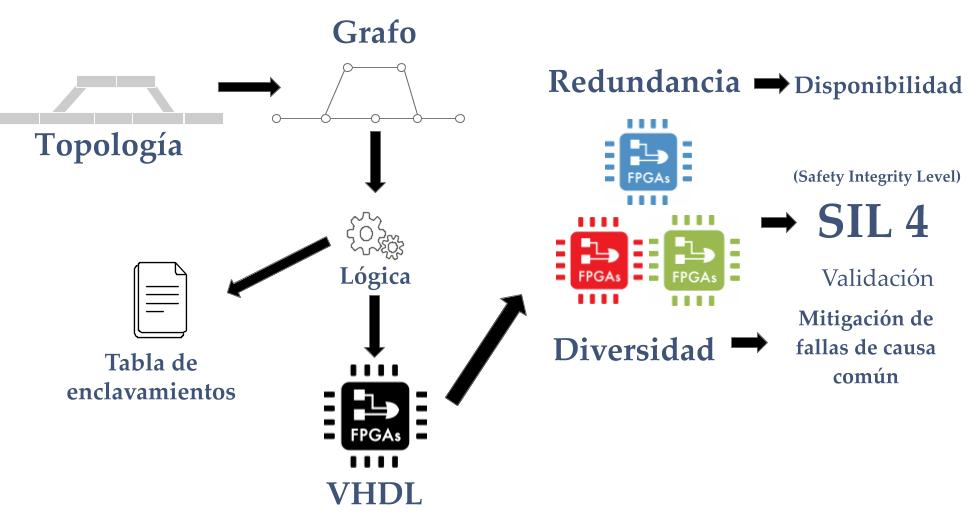
\includegraphics[scale=.4]{./Figures/Geografico_workflow}
			\caption{Esquema de trabajo en el enfoque geográfico.}
			\label{fig:Work_Geografico}
		\end{figure}
	
		A diferencia del enfoque funcional, en el enfoque geográfico la tabla de enclavamientos ocupa un rol secundario al ser un historial del proceso de conversión entre el gráfico y la implementación electrónica del sistema. Obviamente la tabla de enclavamientos del enfoque funcional (al ser incompleta) debe estar contenida en la tabla de enclavamientos del enfoque geográfico (al considerar todas las rutas que admite la red). Ambos enfoques, aunque parten de conceptos distintos, deben converger en los mismos resultados y ser consistentes a la hora de comparar ambas tablas.
		
		El proceso se inicia con el pasaje, de momento manual, del layout al grafo. El cual es analizado por el algoritmo que detecta cuantos semáforos, de cuantos aspectos, en que orientación y donde deben situarse para que el sistema sea seguro. Además de detectar la posición de todos los cambios y barreras, encontrando todas las rutas soportadas por la red y generando una tabla de enclavamientos completa.
		
		El proceso culmina de forma idéntica al enfoque funcional, aplicando estrategias de redundancia y diversidad se buscará alcanzar un nivel de seguridad alto propio de la industria nuclear o aeroespacial.
		
		\subsection{Escalabilidad de la estrategia}	
			
			Realizando el mismo análisis de escalabilidad se llega a una conclusión muy diferente respecto al otro enfoque. Al aumentar la complejidad, y por lo tanto el tamaño, de las topologías, el tamaño de los bloques se mantiene constante, pero aumenta la cantidad de bloques necesarios para implementar el sistema. Esto es ilustrado en la figura \ref{fig:Escala_Geografico}.
					
			\begin{figure}[h]
			\centering
				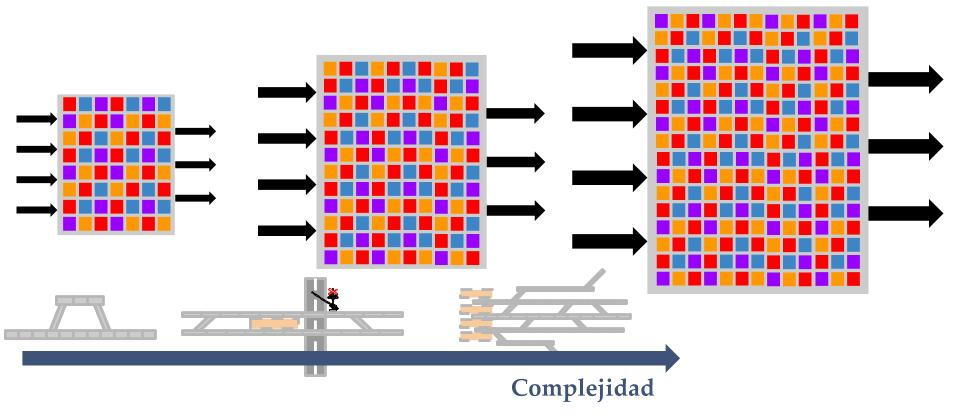
\includegraphics[scale=.4]{./Figures/Geografico_complejidad}
				\caption{Escalabilidad del enfoque geográfico.}
				\label{fig:Escala_Geografico}
			\end{figure}
		
			Todos los tests unitarios, referidos a cada bloque del mismo color que modelan un mismo espacio físico (que puede o no contener una barrera, un cambio o varios semáforos) se elaboran una única vez, sin importar la cantidad de elementos idénticos presentes en la topología. Sumado a que, como en este enfoque se identifican todas las rutas y por lo tanto se pueden generar todos los tests necesarios, entonces la batería de ensayos que otorga este enfoque es completa. Es decir, siempre se tendrán una cantidad de test mayor o igual que la necesaria para cualquier necesidad presente o futura.
		
			Una desventaja de este enfoque es que se debe implementar el analizador de redes ferroviarias y un conversor que dado un grafo genere toda la estructura de archivos necesaria para implementar el circuito electrónico en una FPGA. Por lo tanto, la complejidad y en consecuencia el tiempo de desarrollo es mayor.
			
			
			
